% Титульный лист (ГОСТ Р 7.0.11-2001, 5.1)
\thispagestyle{empty}%
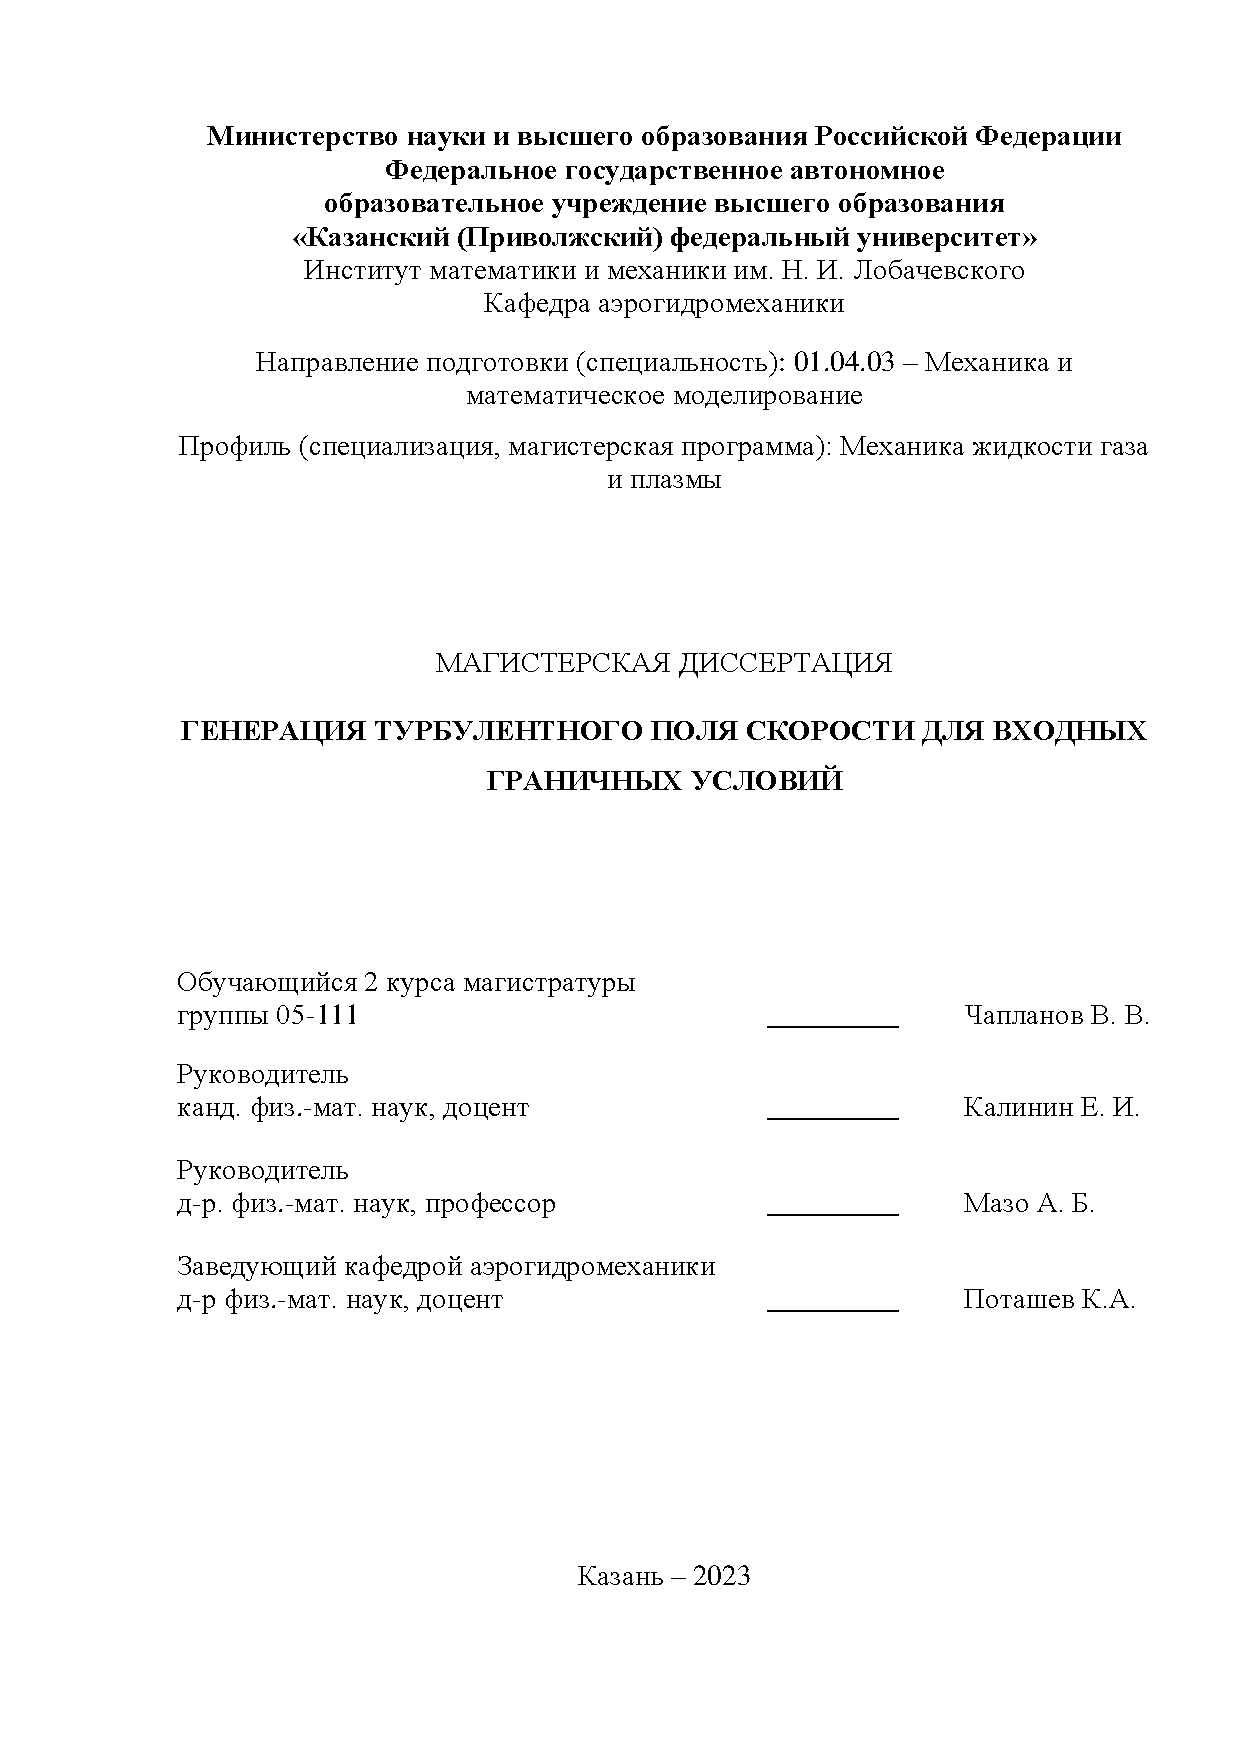
\includepdf{titlepage.pdf}
% \begin{center}%
% \MakeUppercase{
% \textbf{МИНИСТЕРСТВО НАУКИ И ВЫСШЕГО ОБРАЗОВАНИЯ РОССИЙСКОЙ ФЕДЕРАЦИИ
% Федеральное государственное автономное образовательное учреждение высшего образования «КАЗАНСКИЙ (ПРИВОЛЖСКИЙ) ФЕДЕРАЛЬНЫЙ УНИВЕРСИТЕТ»
% Институт математики и механики им. Н.И. Лобачевского
% Кафедра аэрогидромеханики
% }}
% \end{center}%
% %
% \vspace{0pt plus4fill} %число перед fill = кратность относительно некоторого расстояния fill, кусками которого заполнены пустые места

% Направление подготовки (специальность): 01.04.03 - Механика и математическое моделирование

% Профиль (специализация, магистерская программа): Механика жидкости газа и плазмы

% \vspace{0pt plus4fill}
% \begin{center}%
%     \MakeUppercase{Магистерская диссертация}
% \end{center}%

% \vspace{0pt plus4fill}
% \begin{center}%
%     \MakeUppercase{Генерация турбулентного поля скорости для входных граничных условий}
% \end{center}%

% \begin{flushright}%
% На правах рукописи

% \textsl {УДК \thesisUdk}
% \end{flushright}%
% %
% \vspace{0pt plus6fill} %число перед fill = кратность относительно некоторого расстояния fill, кусками которого заполнены пустые места
% \begin{center}%
% {\large \thesisAuthor}
% \end{center}%
% %
% \vspace{0pt plus1fill} %число перед fill = кратность относительно некоторого расстояния fill, кусками которого заполнены пустые места
% \begin{center}%
% \textbf {\large \thesisTitle}

% \vspace{0pt plus2fill} %число перед fill = кратность относительно некоторого расстояния fill, кусками которого заполнены пустые места
% {%\small
% Специальность \thesisSpecialtyNumber~---

% <<\thesisSpecialtyTitle>>
% }

% \vspace{0pt plus2fill} %число перед fill = кратность относительно некоторого расстояния fill, кусками которого заполнены пустые места
% Диссертация на соискание учёной степени

% \thesisDegree
% \end{center}%
% %
% \vspace{0pt plus4fill} %число перед fill = кратность относительно некоторого расстояния fill, кусками которого заполнены пустые места
% \begin{flushright}%
% Научный руководитель:

% \supervisorRegalia

% \supervisorFio
% \end{flushright}%
% %
% \vspace{0pt plus4fill} %число перед fill = кратность относительно некоторого расстояния fill, кусками которого заполнены пустые места
% \begin{center}%
% {\thesisCity~--- \thesisYear}
% \end{center}%
\newpage
